
\documentclass{beamer} 
\usepackage{blindtext, graphicx}
\usepackage[utf8]{inputenc}

\usepackage{enumerate}

% Citation
%\usepackage{cite}

% Graphics
\usepackage{graphicx}
\graphicspath{{images/}}
\usepackage{subfigure}
\DeclareGraphicsExtensions{.pdf,.jpeg,.png,.eps}
\usepackage{booktabs}

% Math
%\usepackage[cmex10]{amsmath}

% Urls
\usepackage{url}

% Tables
\usepackage{booktabs}

% Optional packages
%\usepackage{array}
%\usepackage{mdwmath}
%\usepackage{mdwtab}
%\usepackage{eqparbox}
%\usepackage[tight,footnotesize]{subfigure}
%\usepackage[caption=false]{caption}
%\usepackage[font=footnotesize]{subfig}
%\usepackage[caption=false,font=footnotesize]{subfig}

% correct bad hyphenation here
%\hyphenation{op-tical net-works semi-conduc-tor}





\usepackage{res/theme/beamerthemeExecushares}
\usepackage[style=numeric]{biblatex}
\setbeamertemplate{bibliography item}{\insertbiblabel}
\bibliography{presentation}


%\setbeamertemplate{bibliography item}{\insertbiblabel}


\newcommand {\framedgraphic}[2] {
	\begin{frame}{#1}
	\begin{center}
		\includegraphics[width=\textwidth,height=0.8\textheight,keepaspectratio]{#2}
	\end{center}
\end{frame}
}


\setlength{\abovecaptionskip}{0pt plus 3pt minus 2pt}
\setlength{\belowcaptionskip}{0pt plus 3pt minus 2pt}



\hfuzz=100pt
\vfuzz=100pt


\setcounter{showSlideNumbers}{1}



\title{Impact of HEVC encoding presets for resolutions up to UHD-1}
\author{Christopher Krämmer \inst{1} \and Serge Molina \inst{2} \and Anton Schubert \inst{1}}
\institute[shortinst]{\inst{1} Institute for Media Technology, TU Ilmenau for Christopher Krämmer \and \inst{2} Systèmes Robotiques et Interactifs UPSSITECH for Serge Molina}

\begin{document}



\setcounter{framenumber}{-1}
\setcounter{showProgressBar}{1}
\setcounter{showSlideNumbers}{0}
\frame{\titlepage}


\begin{frame}
	\frametitle{Introduction}
	Online video streaming accounts for a large amount of Internet traffic. To adapt better to changing bandwidth requirements more and more content distributors employ HTTP Adaptive Streaming (\textit{HAS}), however the present availability of specific quality measures is not adequate. This paper aims for linking predicted quality and subjective user ratings based on the \textit{VMAF} metric and an \textit{ACR}-style experiment. Therefore, we analyzed encodings of six different 10-second sequences at varying resolutions up to \textit{UHD-1} with three bitrates per resolution and compared the results with ratings from the perceptual test based on a "na\"{\i}ve" and an "expert" encoding preset. Subsequently, we found that we could accurately predict our final subjective quality results using the \textit{VMAF} metric. Our aggressive optimization with the "expert" encoding preset saved bits and preserved quality at higher bitrates, but lead to visual quality degradation for low bitrates.
\end{frame}


\setcounter{framenumber}{-1}
\setcounter{showProgressBar}{1}
\setcounter{showSlideNumbers}{0}
\begin{frame}
\frametitle{Contents}
\begin{enumerate}
	\item Test Preparation
	
	\begin{enumerate}
		\item Video Selection
		\item Encoding Parameters
		\item Test Setup
	\end{enumerate}
	
	
	\item Test Results and Analysis
	\begin{enumerate}
		\item Participants population
		\item Collected MOS analysis
		\item Additional data analysis
		\item Regions classification
	\end{enumerate}
	
	\item Conclusion
	
\end{enumerate}
\end{frame}



\section{Test Preparation}
\begin{frame}
	This section will show the different steps followed during the preparation of the subjective experiment. These steps will be described as precisely as possible in order to guarantee reproducibility of our results. 
At first the video selection methodology and the associated sources are introduced in the video selection section. Following that, section \ref{sec:encoding} describes how the source sequences are encoded, and finally section \ref{sec:test_setup} presents the test setup with its dedicated rating framework. 
\end{frame}

\begin{frame}
	\frametitle{Video Selection}
	\begin{frame}
\frametitle{Video Selection}

\large{Preconsiderations for the reference video files}
\begin{itemize}
	
\item Large variety between sequences
\item Captured in UHD-1 or 4k with high quality
\item Length of 10 sec (HAS-segment) with no cut inside
\item Smallest permitted frame rate of 50 fps
\item Colour depth of 10 bit per channel

\end{itemize}

\end{frame}


\begin{frame}
\frametitle{Video Selection}
\large{Dataset Preparation}

\begin{itemize}

\item Database:
\newline Harmonic \cite{web:harmonic}, Cable Labs \cite{web:cablelabs}, Blender Foundation \cite{web:bbb}.	
\item Main challenge: 
\newline Find video sequences with a duration of 10 sec or longer without cuts
\item Preselection with a 4k screen:
\newline Find visual artefacts and select reference video files with a large variety between them

\end{itemize}
\end{frame}


\begin{frame}
\frametitle{Video Selection}

\begin{figure}[hbt!]
	\begin{center}
		%
		
		\subfigure[Air Show]{%
			\label{fig:airshow}
			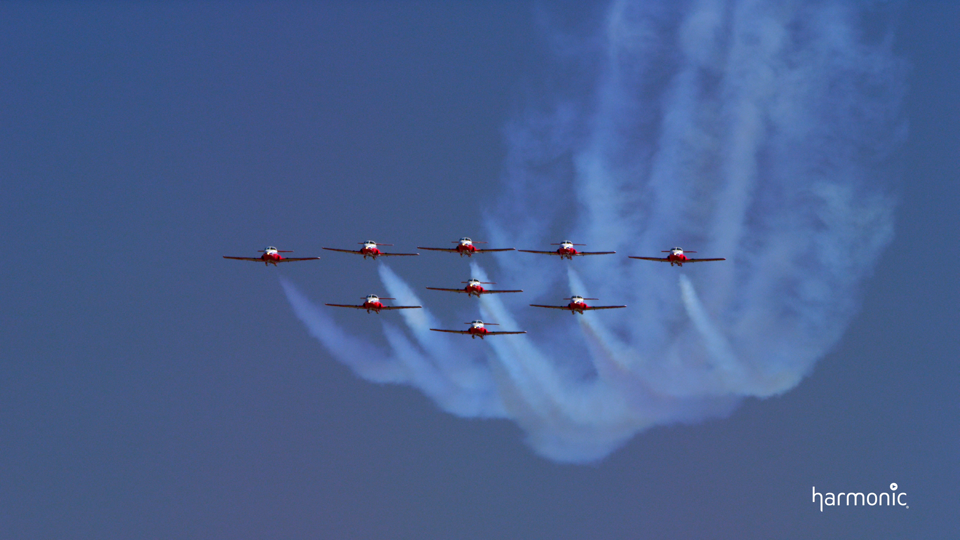
\includegraphics[width=0.3\textwidth]{images/AirShow}
		}%
		\subfigure[Big Buck Bunny]{%
			\label{fig:bbb}
			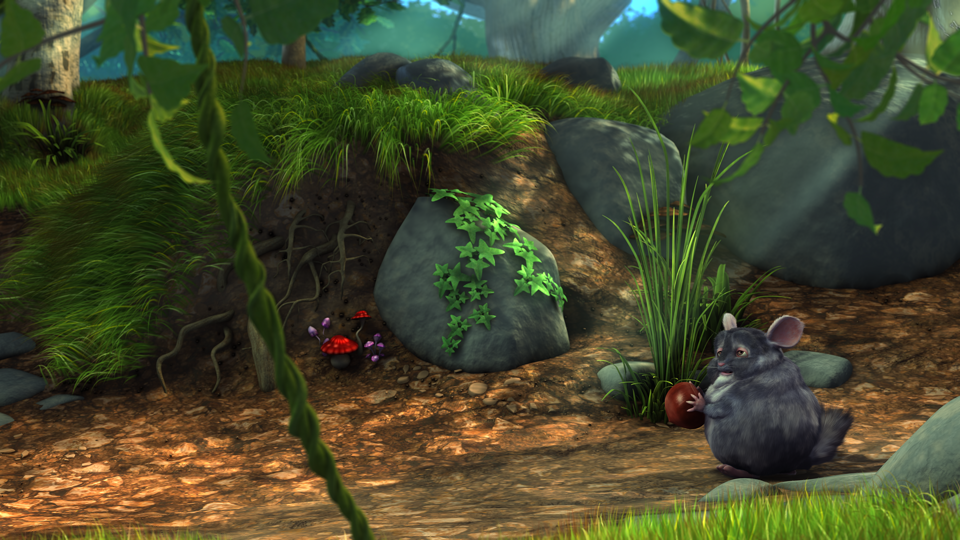
\includegraphics[width=0.3\textwidth]{images/Bbb}
		}
		\subfigure[Fjord]{%
			\label{fig:Fjord}
			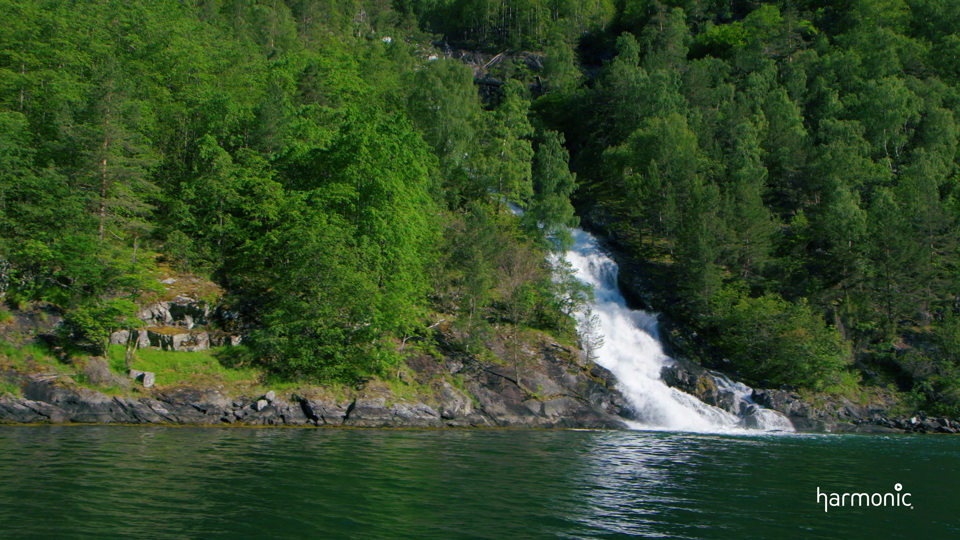
\includegraphics[width=0.3\textwidth]{images/Fjord}
		}\\ %  ------- End of the first row ----------------------%
		\subfigure[Moment of Intensity]{%
			\label{fig:MomentOfIntensity}
			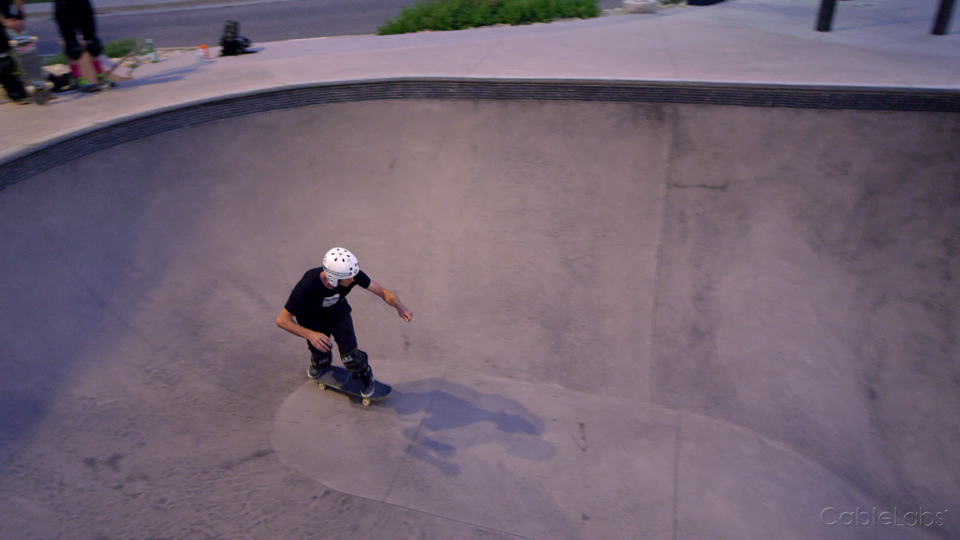
\includegraphics[width=0.3\textwidth]{images/MomentOfIntensity}
		}		
		\subfigure[Snow Monkeys]{%
			\label{fig:SnowMonkeys}
			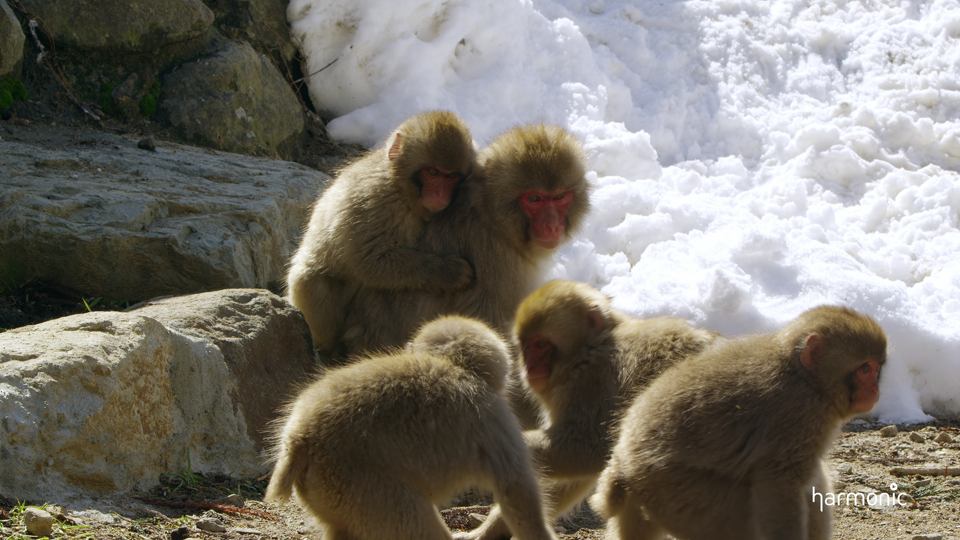
\includegraphics[width=0.3\textwidth]{images/SnowMonkeys}
		}%
		\subfigure[Streets of India]{%
			\label{fig:StreetsOfIndia}
			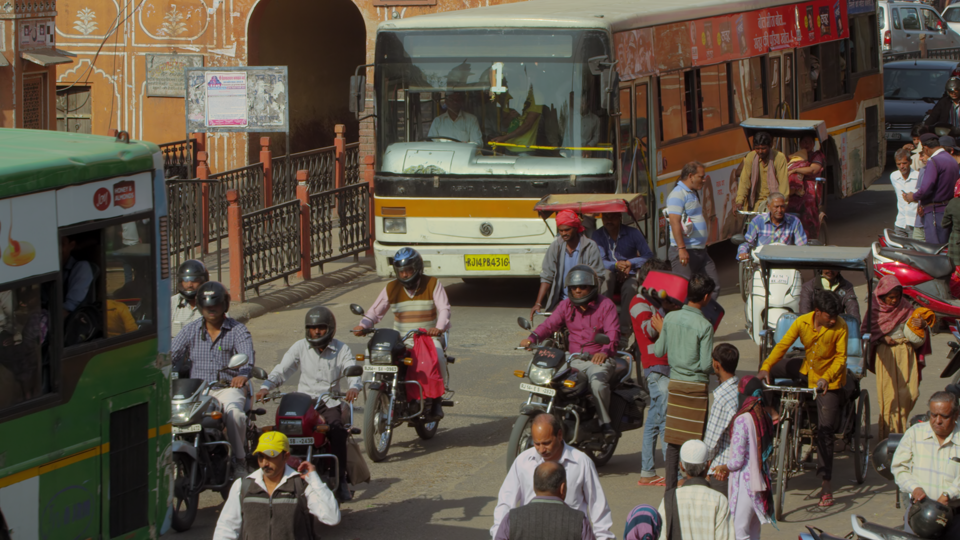
\includegraphics[width=0.3\textwidth]{images/StreetsOfIndia}
		}%
		%
	\end{center}

\end{figure}

Selection of frames contained in the reference videos to show the variety of the content.
\end{frame}


\begin{frame}
\frametitle{Video Selection}

\begin{figure}[hbt!]
	\centering
	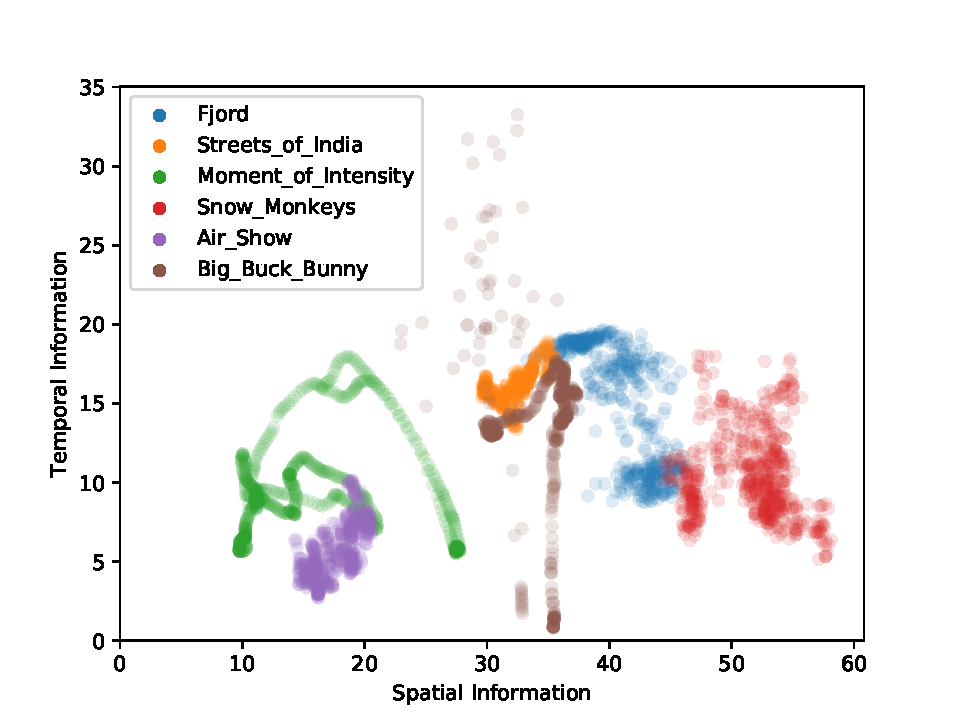
\includegraphics[width=2.9in]{SITI}
\end{figure}

Spatial and temporal information of the reference video files.
\newline Each dot represents one frame.


\end{frame}



\end{frame}

\begin{frame}
	\frametitle{Encoding Parameters}
	\label{sec:encoding}
	As one of the focus points of this paper the choice of encoding parameters and the video preprocessing are of main importance. This section will first cover the two different encoding presets, go over the method which is used to derive the target bitrates and finalize with a description of the process automation.

\large{Encoding Presets}
We use the open x265 encoder for our experiment as it offers good performance and integration in the FFmpeg toolchain. Two different presets are used for the sequence encodings, a "na\"{\i}ve" (1) and an "expert" preset (2). The "na\"{\i}ve" preset is a simple \textit{CBR} (Constant Bitrate) encoding, whereas the "expert" preset is a 2-pass encoding with a Quality-Control pass followed by a Bitrate-Control pass.  Every sequence is encoded with both presets at 3 resolutions (540p, 1080p, 2160p) and 3 bitrates for each resolution. The following section goes into detail on how we select those bitrates.

\begin{figure}[thb!]
	\centering
	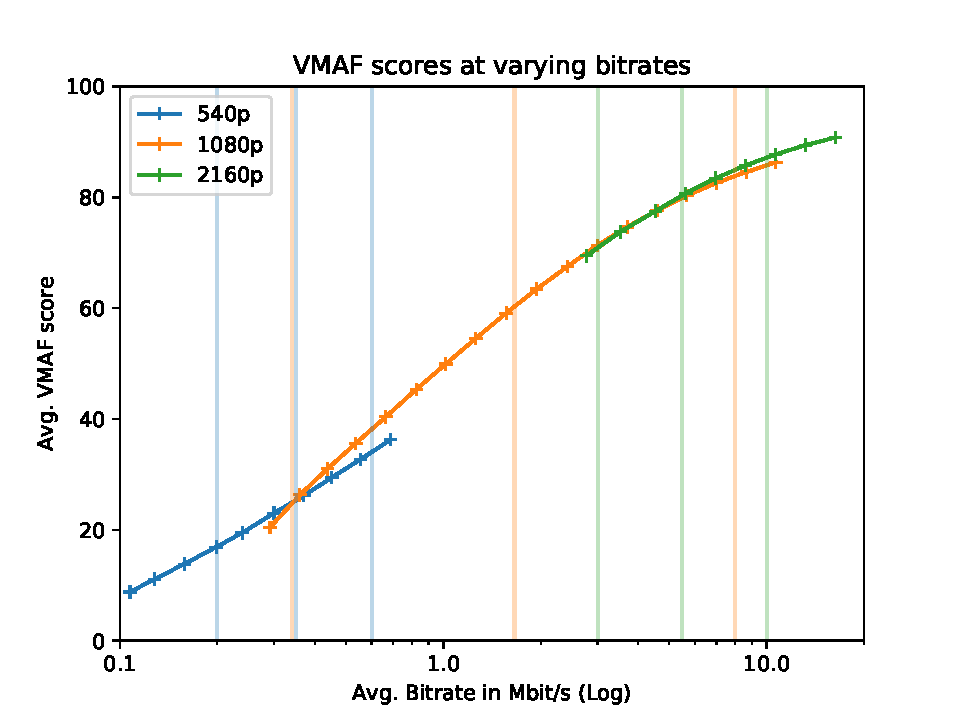
\includegraphics[width=3.5in]{vmaf_bitrates}
	\caption{Average \textit{VMAF} scores for 25 different bitrates at 3 resolutions. The encoded bitrates and the \textit{VMAF} scores are averaged between the 6 sequences and form the abscissa (Log) and ordinate respectively.}
	\label{fig:vmaf:bitrates}
\end{figure}

\large{Selection of Bitrates}
Video Multi-Method Assessment Fusion (\textit{VMAF}) is a full reference metric for estimating human perception of video quality \cite{lin2013:mmf}. We use \textit{VMAF} because it provides a better estimate of subjective quality than single metrics like \textit{SSIM} or \textit{VIF}.

To estimate relevant \textit{HEVC} encoding bitrates for our source content we sample the \textit{VMAF} scores at 25 bitrates on a logarithmic scale for our 3 different resolutions (540p, 1080p, 2160p). The reference sequences are resampled to a fixed 50 frames per seconds to avoid frame rate differences, while the distorted sequences are downsampled, encoded with \textit{CBR} rate control and upsampled to \textit{UHD-1} again using lanczos resampling. Both presets use 4:2:0 chroma subsampling to be close to the typical use-case of webvideo. The sampling requires 222 total sequences to be encoded with x265 and analyzed with the \textit{VMAF Development Kit} (VDK). This process takes around 18 hours (excluding download and cutting of the source material) on a current 10-Core x64 CPU.

The resulting \textit{VMAF} scores exhibit an overlap between different resolutions and the final encoding bitrates are chosen near those intersections. Figure \ref{fig:vmaf:bitrates} shows the sampled scores with the target rates in the background. We choose the target bitrates at least 2 bitrate-samples away from an intersection with the next quality, except for the lower 1080p-bound where it is not possible to lower the bitrate any further due to encoder restrictions. This should ensure a relevant sampling of the \textit{MOS}-bitrate space for the subjective test.

\begin{figure}[thb!]
	\centering
	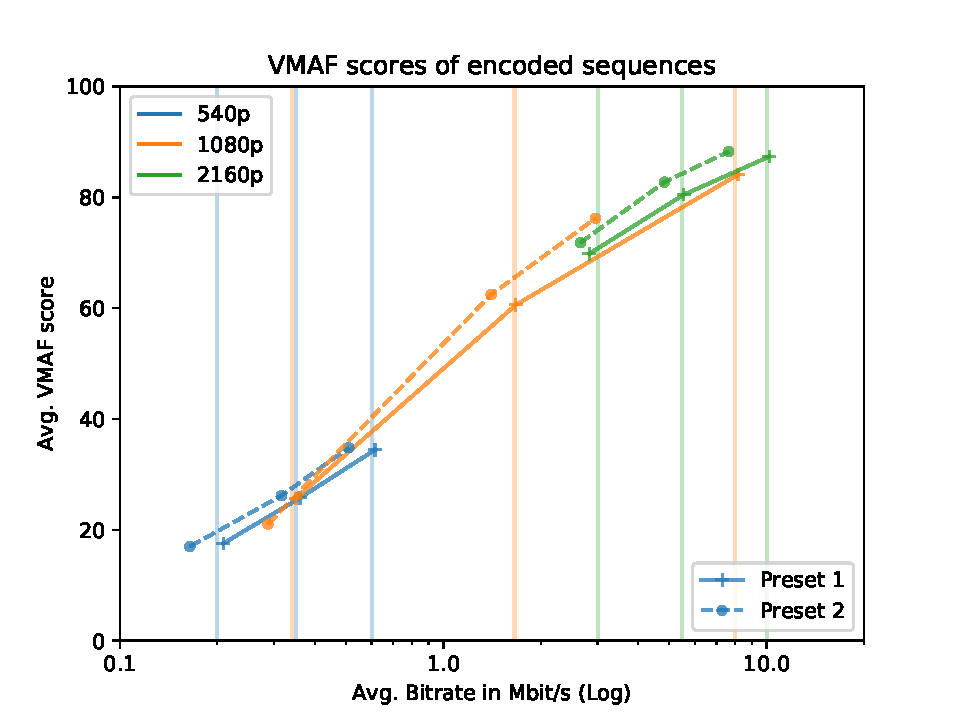
\includegraphics[width=3.5in]{vmaf_final}
	\caption{Average \textit{VMAF} scores of encoded videos for both presets. The encoded bitrates and the \textit{VMAF} scores are averaged between the 6 sequences for each preset and form the abscissa (Log) and ordinate respectively.}
	\label{fig:vmaf:encoded}
\end{figure}

The average \textit{VMAF} scores of the two presets at the chosen bitrates can be seen in Figure \ref{fig:vmaf:encoded}. The respective target bitrates can be seen in the background again. The scores of the "expert" preset (2) are consistently higher than the ones for the "na\"{\i}ve" preset (1) at matching target bitrates. Furthermore, the "expert" preset saves bitrate by resorting to an acceptable level of quality, while the "na\"{\i}ve" presets bitrates are very close to the targets. However, we can see that the preset two sometimes reduces the bitrate too far so that the average score is well below preset one. This happens especially for the lowest 1080p bitrate and less so for the 540p encodings.


\begin{figure}[bht!]
	\centering
	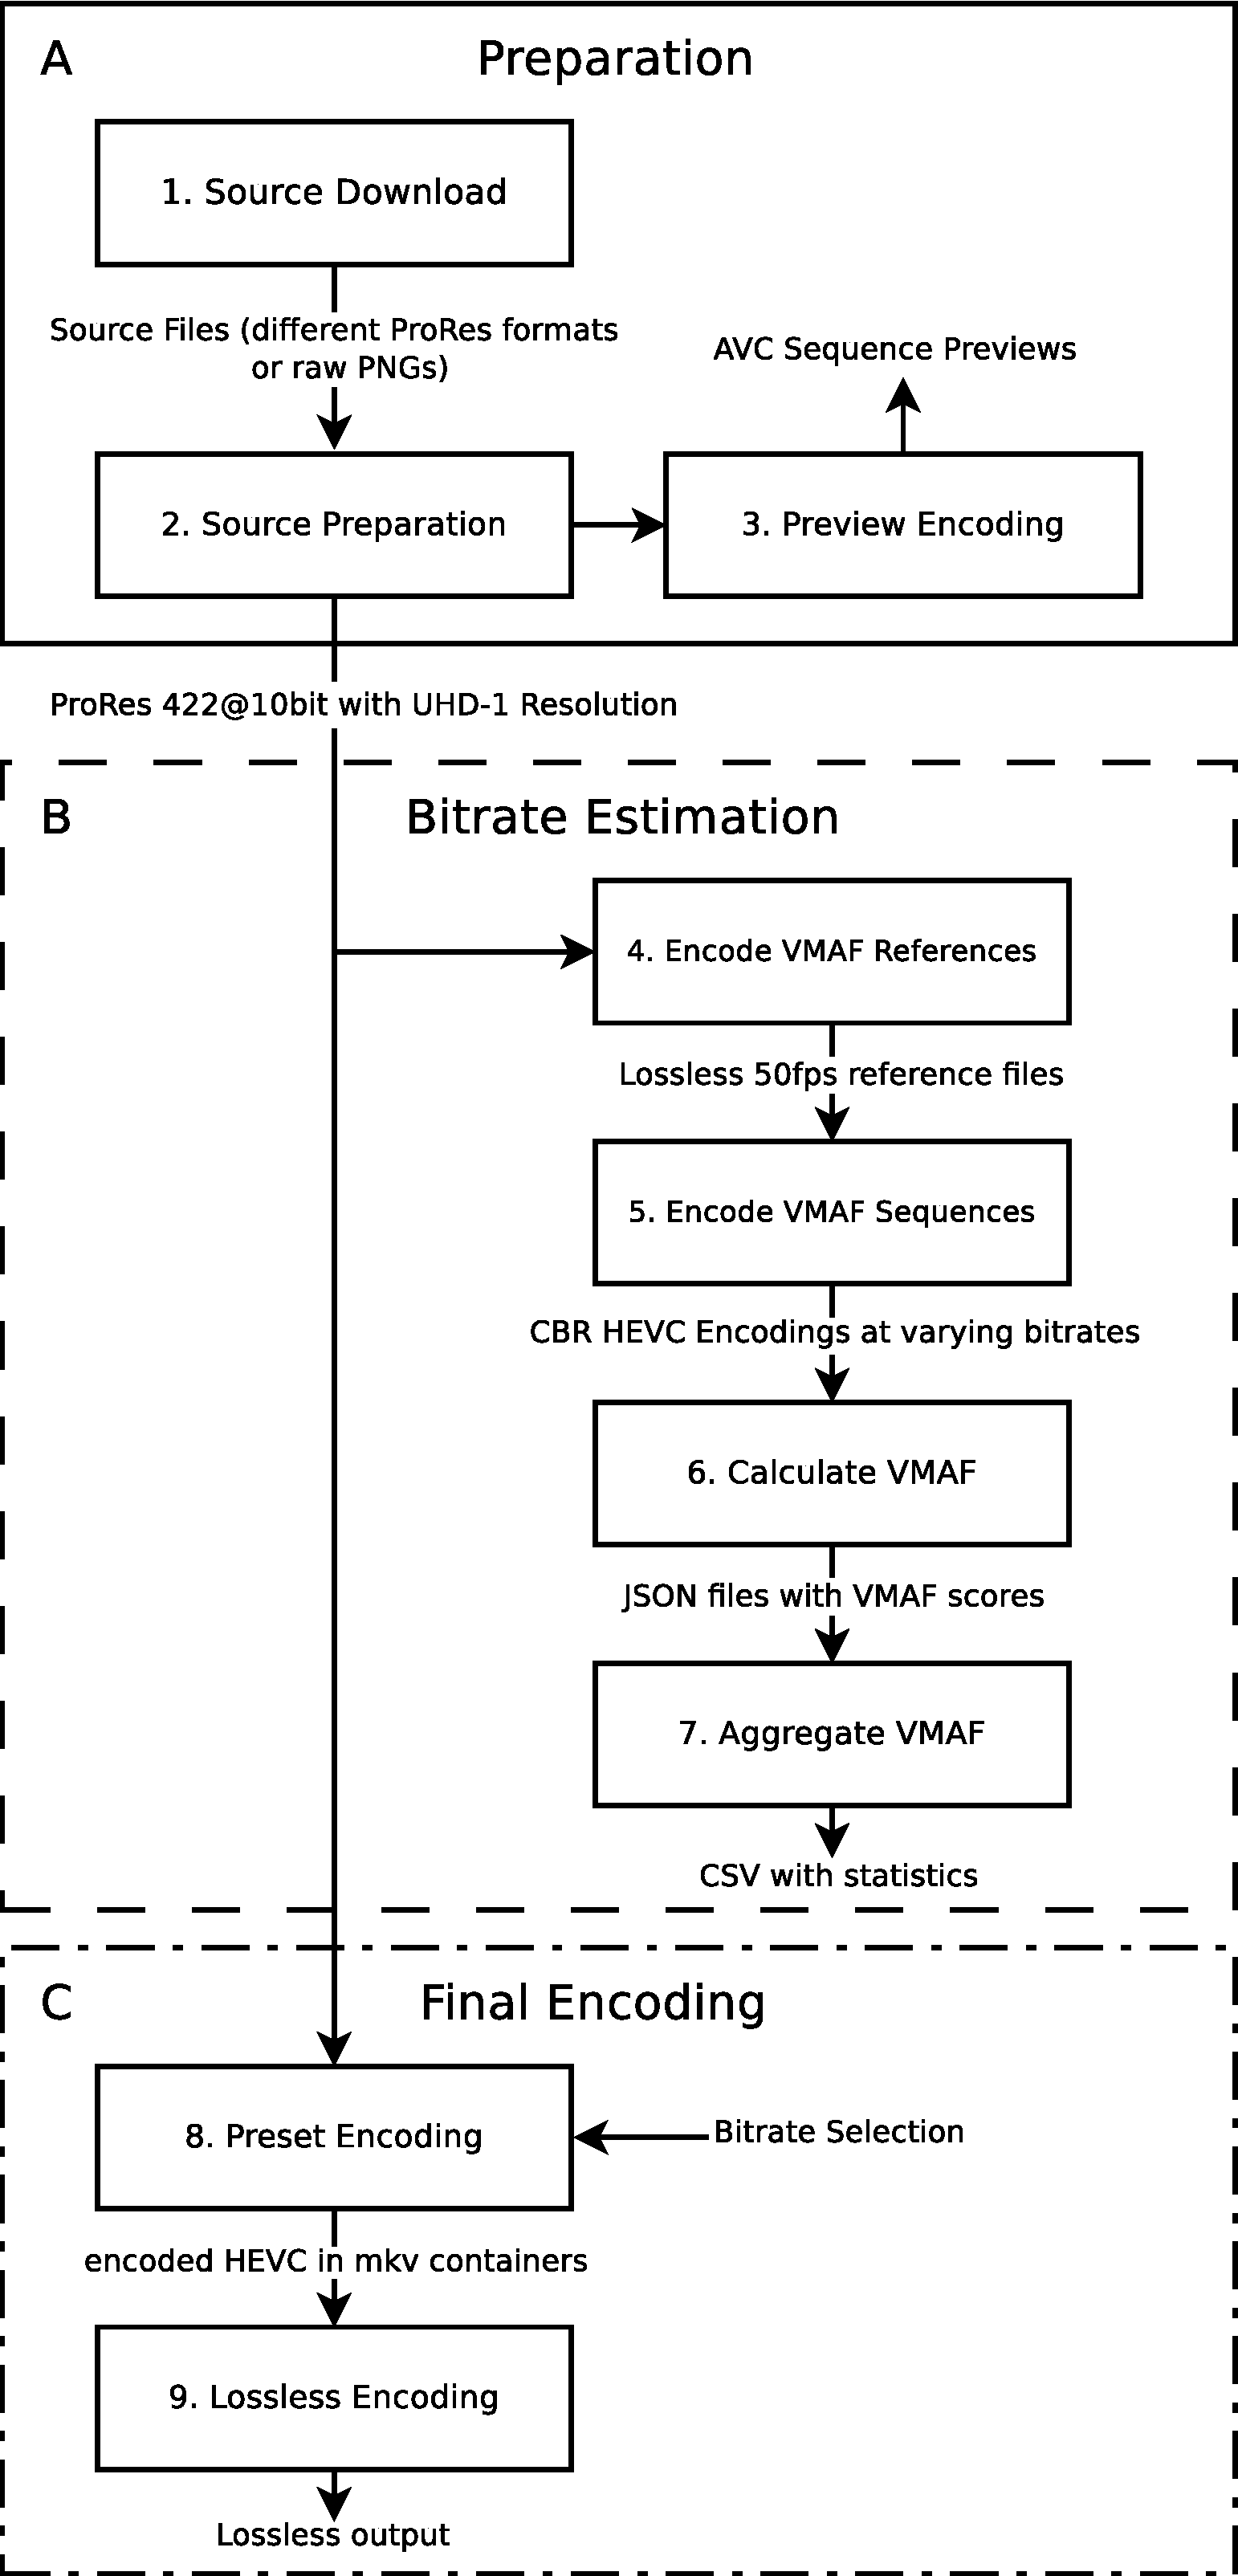
\includegraphics[width=2.5in]{automation}
	\caption{Automated processing and encoding workflow.}
	\label{fig:automation}
\end{figure}

\large{Encoding Automation}
We automate the whole process for downloading, preprocessing and encoding the source videos using pydoit \cite{web:pydoit}. This speeds up the turnaround time for changed parameters or sequences and also ensures that the encoded material can later be reproduced.

The whole process is illustrated in Figure \ref{fig:automation} and starts with the source preparation (A). After download of the sequences (1) they are cut to 10 seconds length and saved as ProRes HQ with \textit{UHD-1} resolution (2). Additionally, \textit{MPEG4-AVC} previews are generated at a lower resolution of 1440p to allow review of the sequences on slower devices.

After the initial processing the bitrate estimation is performed (B) using the \textit{VMAF} metric \cite{lin2013:mmf}. The videos are brought to the same frame rate of 50fps (4) and encoded with \textit{CBR} at 25 different bitrates (5). The average \textit{VMAF} score of each video is analyzed with the \textit{VMAF} Development Kit (VDK) \cite{web:vdk} and saved as a json file (6). All of the average scores are then aggregated into a single CSV for plotting and further analysis (7). The target bitrates can then derived from these scores.

The last step is the main encoding (C). It can only start after the target bitrates have been specified in the configuration. The sequences are encoded first with the two presets (8) and transcoded to a lossless format (ffvhuff) afterwards, to allow for fast and consistent playback as well as archiving of the video material.



\end{frame}

\begin{frame}
	\frametitle{Test Setup}
	\label{sec:test_setup}
	Several steps have been followed in order to enable the acquisition of meaningful data during the subjective tests. These steps include defining the test environment, choosing a rating framework and creating additional question that may help inferring informations about the participants and their way of rating content.


\large{Test Environment}
In order to make the results of our research reproducible we follow the ITU P.910 \cite{rec1998p} recommendation. 
The parameters include aspects such as viewing distance, peak luminance of the screen or background room illumination.
Performing tests following these specifications is common at the Technical University of Ilmenau, so we used a room meeting these requirements, which was already available.


	
\large{Rating Framework}
The testing procedure which seems most suited to this case is Absolute Category Rating (ACR) \cite{rec1998p}, where different versions of an original sequence are shown to a test participant. 

For each sequence the participant issues categorical ratings from any of these 5 answers: \{Excellent, Good, Fair, Poor, Bad\}

The steps performed by a participants during a rating session can be seen in the figure \ref{fig:workflow:state_machine}.

\begin{figure}[htb!]
	\centering
	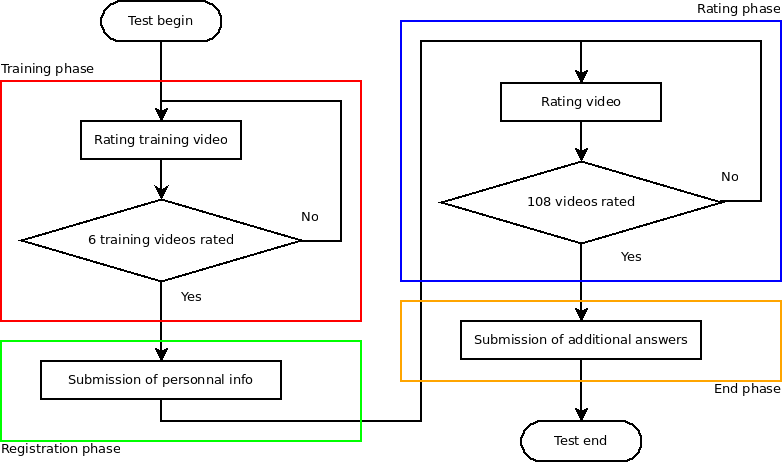
\includegraphics[width=3.5in]{rating_workflow}
	\caption{Detailed steps of a rating session}
	\label{fig:workflow:state_machine}
\end{figure}


\large{Additional collected data}
In order to gain more knowledge about the users behaviour, additional data is collected from the participants.

One of the suggestions of the ITU recommendation paper being the usage of several test questions in addition to the ratings \cite{rec1998p}, the following points have been assessed at the end of each rating session:
\begin{itemize}
	\item Impact of the following points on rating 
	\begin{itemize}
		\item Presence of blocky artifacts
		\item Visible bands of colour
		\item Smoothness of the playback
	\end{itemize}
	\item Exposure to 4k content and devices
	\item Confidence of the participant in his ratings
\end{itemize}

The idea behind these question is dual as they may translate how users perceive video features as well as how users may clearly express their perceptions. As it has been noticed in previous experiments and in discussions with test participants: users may still rate using a different scales, thus spreading the final \textit{MOS} or falsely being classified as outlier when their ratings may only represent a shift from the overall population. 

Moreover, mouse interactions have been collected during the rating of each sequence. The intent behind this is that as the MOS scale forbids detailed answers some participants may hesitate between two answers and change their final answer or hover over several ones before making his final choice.
Answering speed, which could be an indicator of a participant skipping answers or to the contrary being strongly confident in his answers is a feature that has been thought relevant to analyse. 
We believe that informations such as confidence in the participants ratings or more precise scores can be extracted from these previously described behaviours.


\large{Participants selection}
Extra care has been taken during participants selection in order to guarantee unbiased results. This selection process included dividing the participants selection between the different members of the research  group, recruiting participants from different student groups in the University and taking into account participants age and technical background.
\end{frame}



\section{Test Results and Analysis}
\begin{frame}
	This section focuses on presentation and analysis of the result data. At first we look at outliers in our participant data, further analyse the MOS per sequence and per preset and compare the bitrate and quality usage of the preset encodings. Finally we correlate our MOS data with the average \textit{VMAF} scores.
\end{frame}


\begin{frame}
	\frametitle{Participants population}
	\label{sec:participant_population}
	The process of participant selection has allowed recruitment of 26 participants. The distribution of the participants age may be representative of the one from a university campus as seen in figure \ref{fig:participant_population:age_histogram}. We can see that the population still lacks senior participants.

\begin{figure}[htb!]
	\centering
	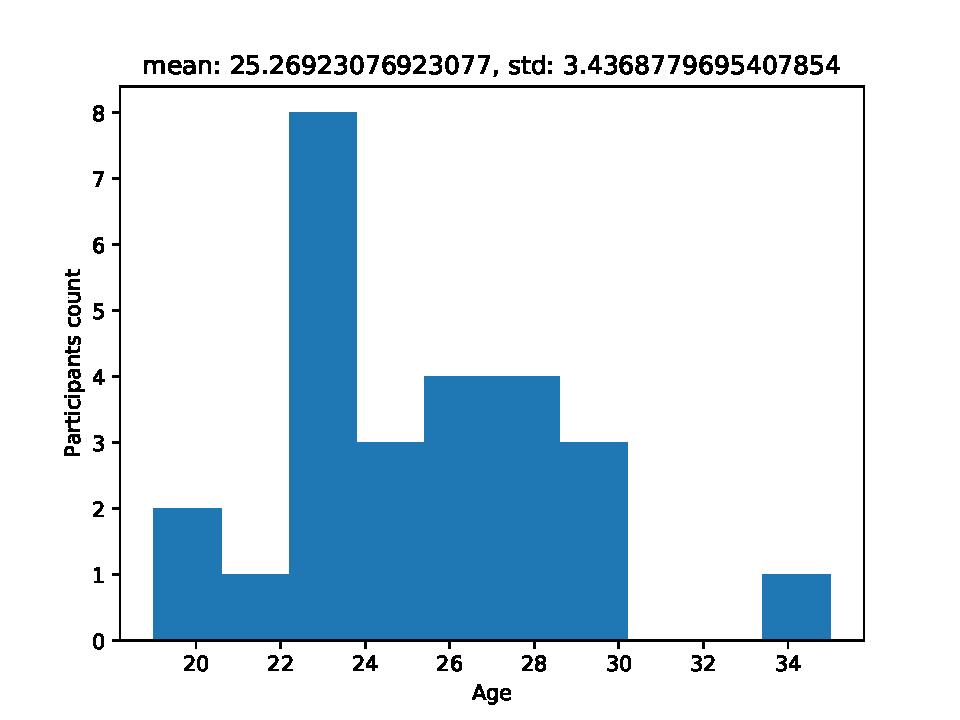
\includegraphics[width=3.5in]{age_histogram}
	\caption{Detailed steps of a rating session}
	\label{fig:participant_population:age_histogram}
\end{figure}

\end{frame}


\begin{frame}
	\frametitle{Collected MOS analysis}
	\label{sec:ratings}
	\begin{frame}
	\frametitle{Collected MOS analysis}
	\large{MOS Outliers}
	\begin{figure}
		\centering
		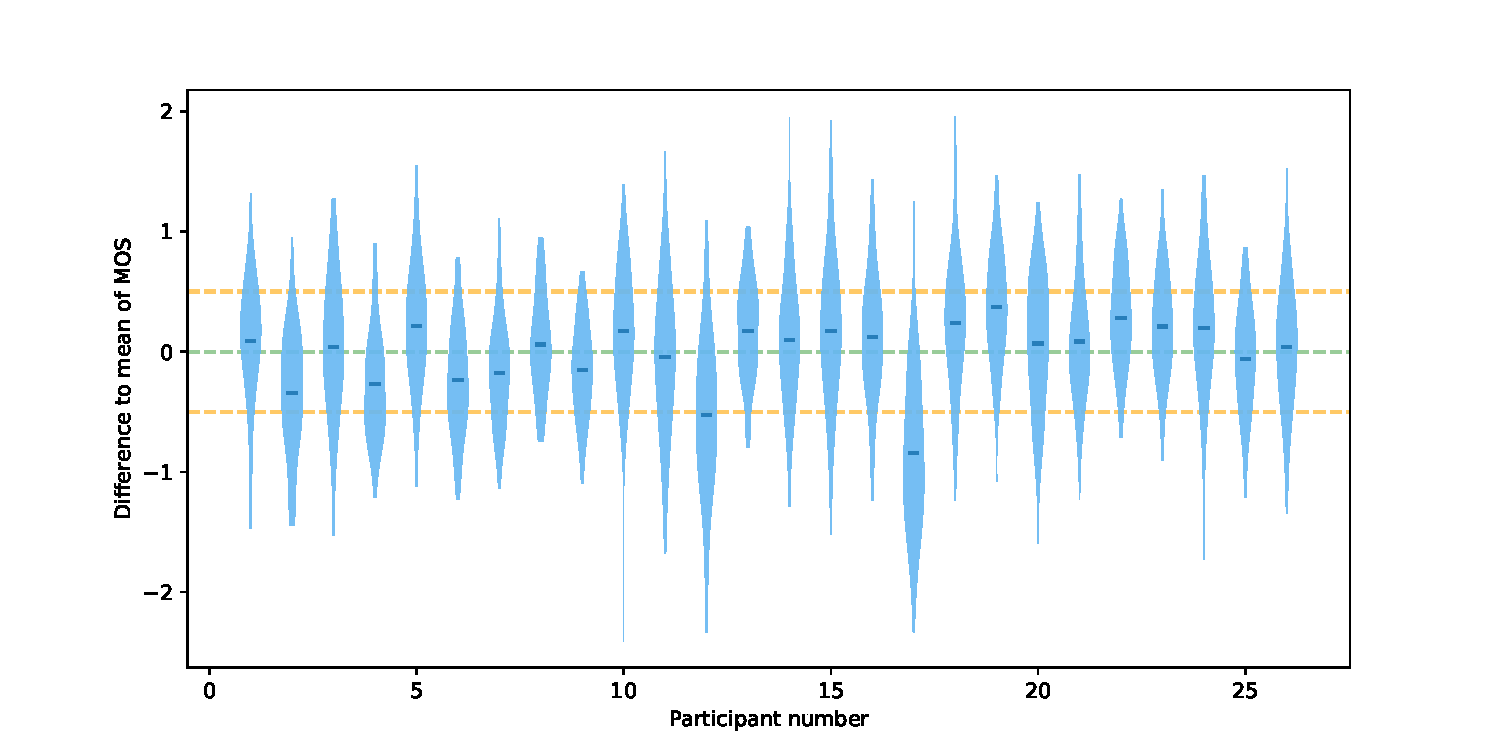
\includegraphics[width=3.7in]{participant_mos_violin}
	\end{figure}

	Difference between average MOS and the invididual ratings for each participant.
\end{frame}

\begin{frame}
	\frametitle{Collected MOS analysis}
	\large{Ratings removal}
	\begin{figure}
		\centering
		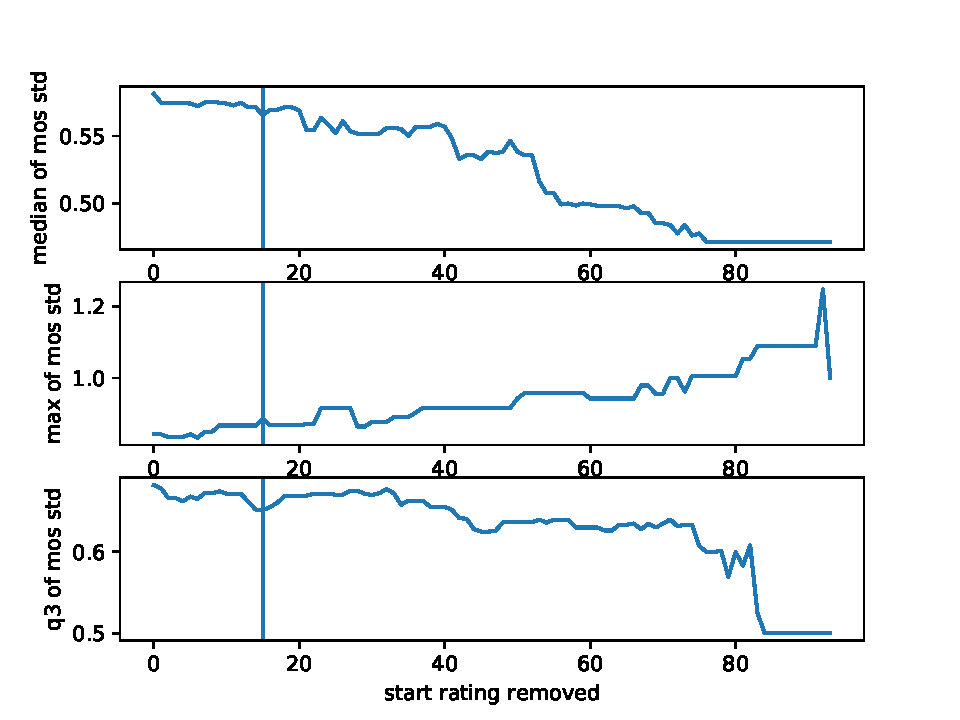
\includegraphics[width=3in]{mos_evolution_per_start}
	\end{figure}
\end{frame}

\begin{frame}
	\frametitle{Collected MOS analysis}
	\large{\textit{MOS} per Sequence}
	\begin{figure}
		\centering
		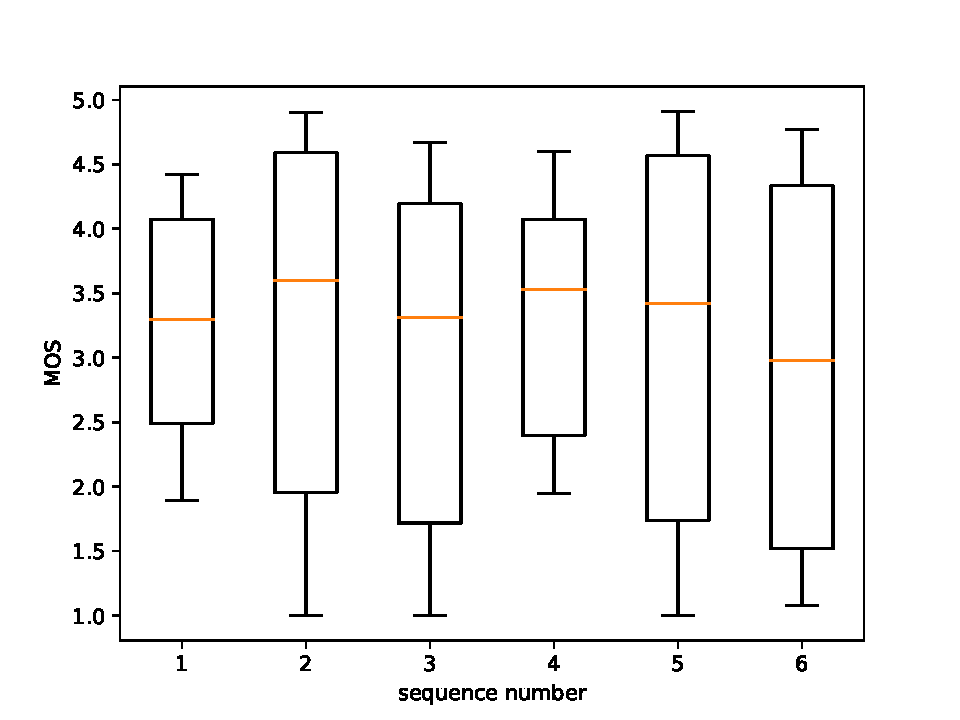
\includegraphics[width=2.6in]{mos_per_sequence}
	\end{figure}

	1: Air Show, 2: Big Buck Bunny, 3: Fjord, 4: Moment of Intensity, 5: Snow Monkeys, 6: Streets of India
\end{frame}

\begin{frame}
	\frametitle{Collected MOS analysis}
	\large{\textit{MOS} per Preset}
	\begin{figure}
		\centering
		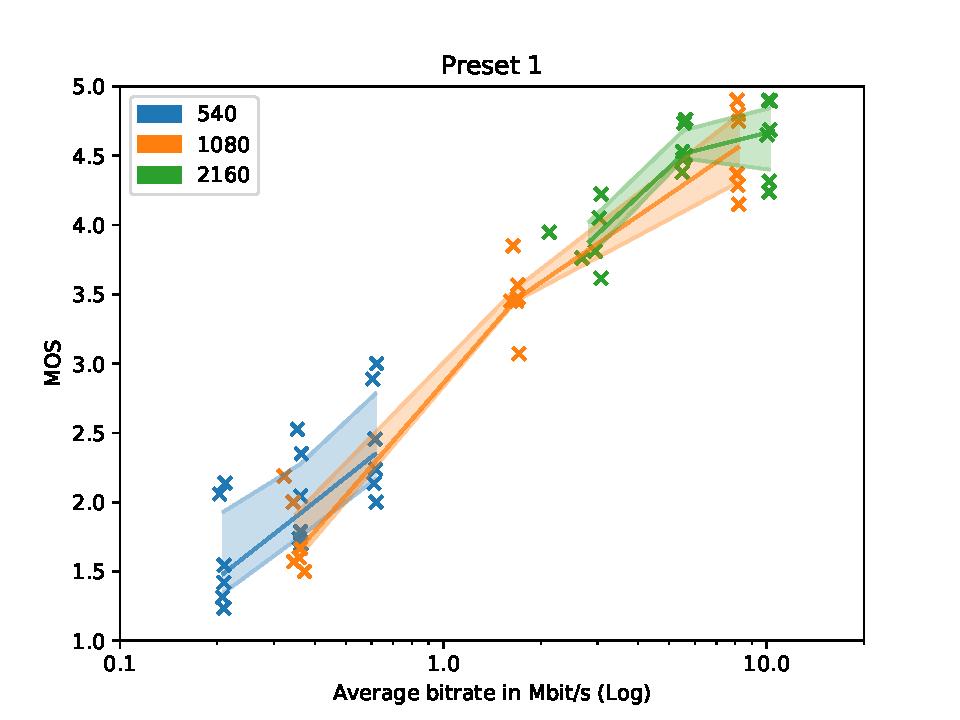
\includegraphics[width=2.25in]{correlation_bitrate_mos_p1}
		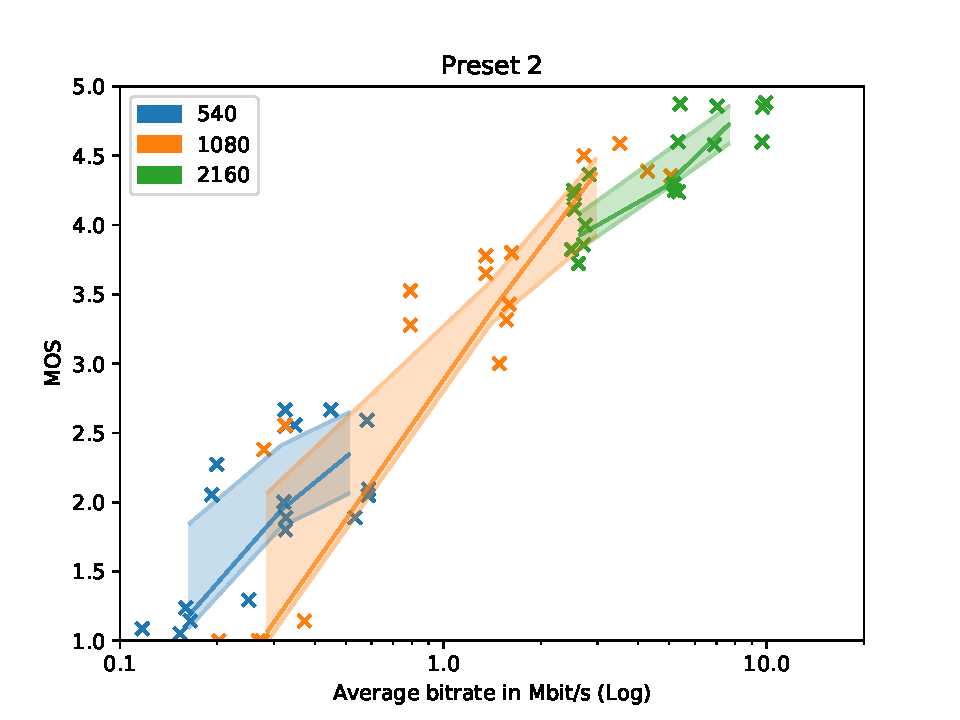
\includegraphics[width=2.25in]{correlation_bitrate_mos_p2}
	\end{figure}
\end{frame}


\begin{frame}
	\frametitle{Collected MOS analysis}
	\large{Preset relative bitrate savings}
	\begin{figure}
		\centering
		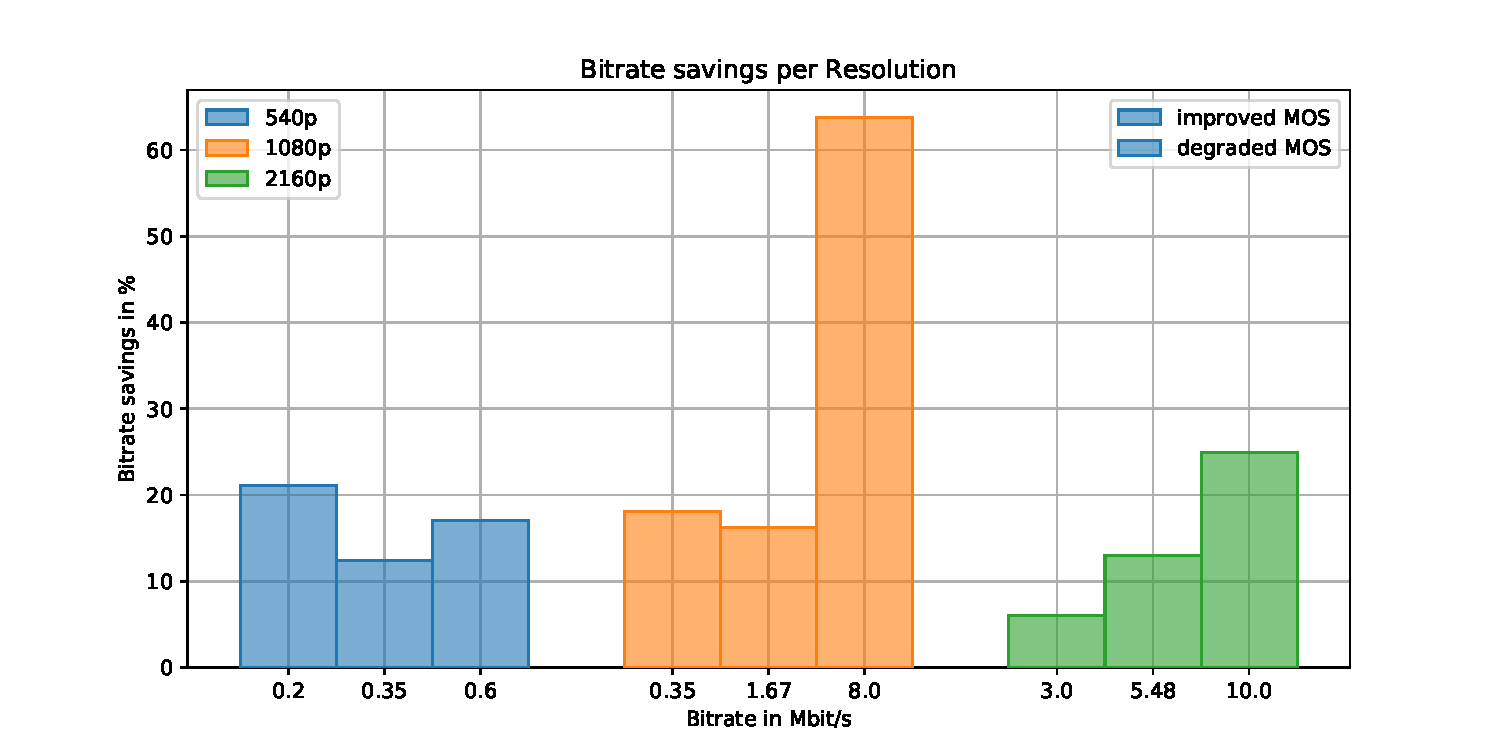
\includegraphics[width=3.7in]{bitrate_savings}
	\end{figure}
\end{frame}

\begin{frame}
	\frametitle{Collected MOS analysis}
	\large{Preset quality difference}
	\begin{figure}
		\centering
		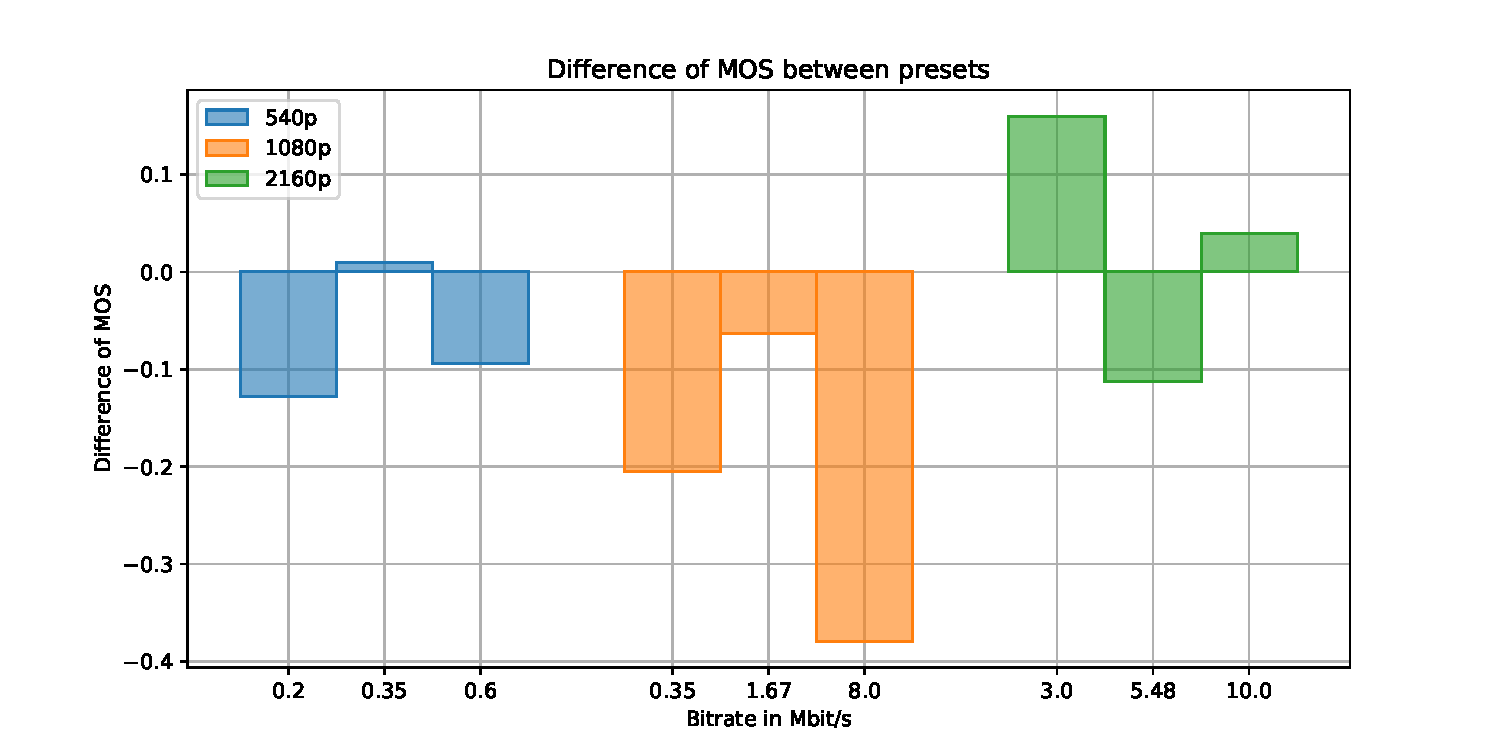
\includegraphics[width=3.7in]{quality_difference}
	\end{figure}
\end{frame}


\begin{frame}
	\frametitle{Collected MOS analysis}
	\large{Correlation between \textit{VMAF} and \textit{MOS}}

	\begin{figure}
		\centering
		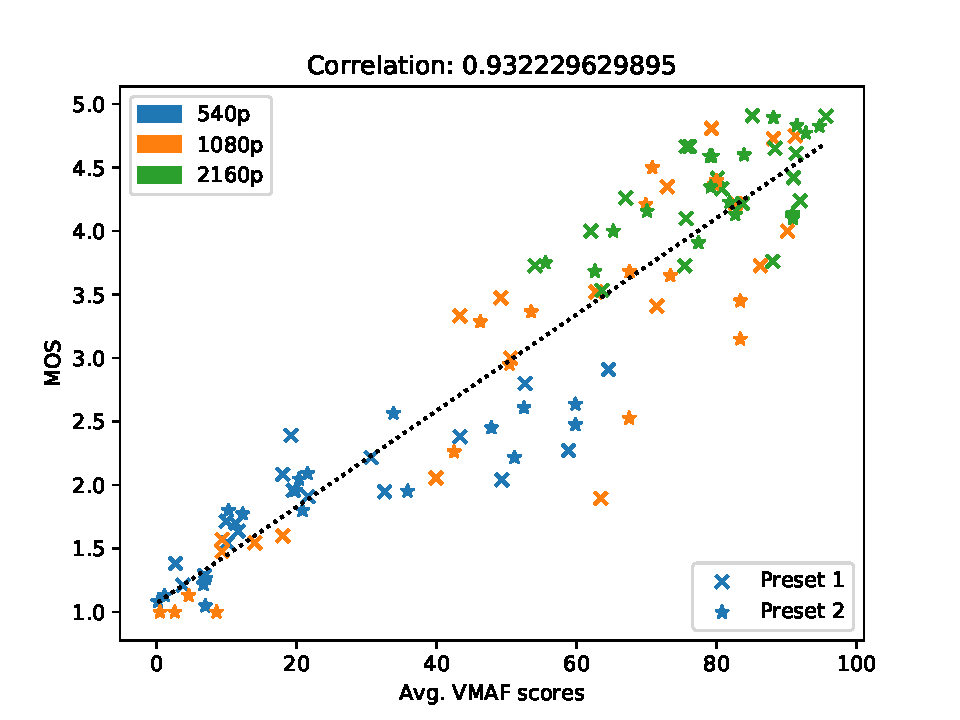
\includegraphics[width=2.8in]{correlation_vmaf_mos}
	\end{figure}
\end{frame}
\end{frame}


\begin{frame}
	\frametitle{Additional data analysis}
	\label{sec:features}
	
\label{sec:additional_data}
Correlation between answers to the feedback questions and the ratings values and characteristics have been computed. These correlations were not significant enough to be further analysed. Although mouse movements was collected, it has not been analysed.
\end{frame}


\section{Conclusion}

\begin{frame}
	\large{Conclusion}
We found that we can predict the be accurately predicted using the \textit{VMAF} metric.
Our aggressive optimization approach with the "expert" encoding preset pays off at higher bitrates but degrades visual quality for low bitrates. This suggests that high-effort multi-pass encodings like ours mainly benefit high resolution content at large bitrates, where the absolute gain can also be larger.


\large{Future Work}
Improvements of the automation framework: the source preparation step could directly transcode the original material to a constant framerate and colour-subsampling in a lossless format to avoid a further preprocessing step for the VMAF metrics.
As we have seen in section \ref{sec:additional_data}, mouse behaviour and user feedback hasn't been analysed as deeply as desired. 
Deeper analysis may be performed in a revision of this paper or another more complete one.

%A longer test or a sectioned test with more participants would provide a better sampling of the bitrate-MOS space and allow for more detailed analysis.

A similar experiment could be done with a specific focus on content-specific encoding approaches like \cite{cock:2016:titleencode}.


\end{frame}
%\appendices
%\section{Proof of the First Zonklar Equation}

% use section* for acknowledgement
%\section*{Acknowledgment}
%The authors would like to thank...

% trigger a \newpage just before the given reference
% number - used to balance the columns on the last page
% adjust value as needed - may need to be readjusted if
% the document is modified later
%\IEEEtriggeratref{8}
% The "triggered" command can be changed if desired:
%\IEEEtriggercmd{\enlargethispage{-5in}}

% References
\printbibliography

\end{document}


